\section{Fundamentals and Related Work} \label{fundamentals}

\subsection{Basics from Molecular Biology} \label{fundamentalsA}

\subsubsection{Genome Sequences} \label{fundamentalsAa}

\begin{wrapfigure}{R}{6cm}
	\centering
	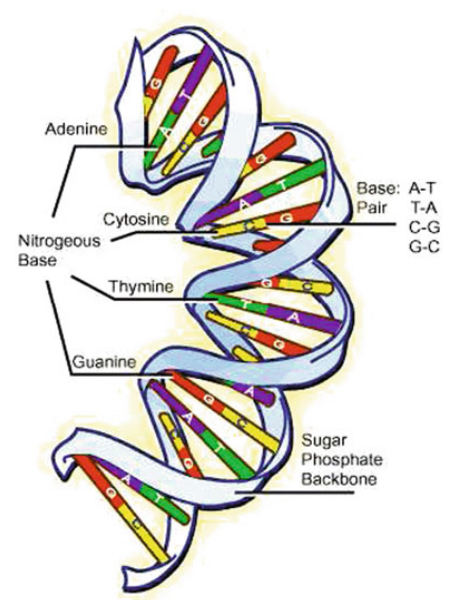
\includegraphics[width=0.9\linewidth]{figures/dnaDoubleHelix.png}
	\caption{\ac{DNA} double helix \cite[p. 8]{10.5555/1965281}}
	\label{dna_double_helix}
\end{wrapfigure}

The human genome is encoded as \ac{DNA}. The \ac{DNA} carries genetic instructions on how \ac{DNA} based organisms develop and behave. It is structured as a double helix and consists of two nucleotide pair combinations: adenine (A), thymine (T) and cytosine (C), guanine (G). \cite[p. 8]{10.5555/1965281}

%\begin{figure}[ht]
%	\centering
%	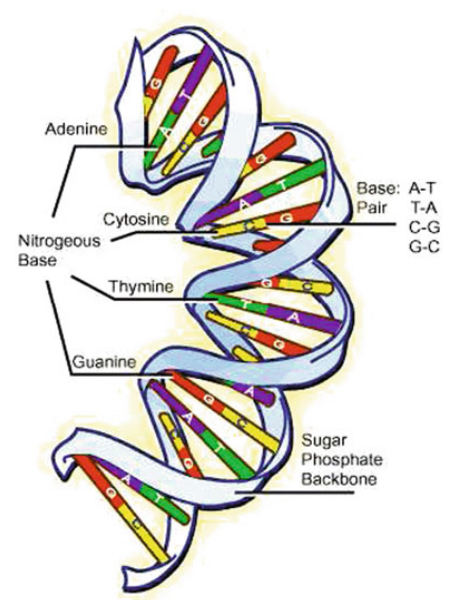
\includegraphics[width=0.35\linewidth]{figures/dnaDoubleHelix.png}
%	\caption{\ac{DNA} double helix \cite[p. 8]{10.5555/1965281}}
%	\label{dna_double_helix}
%\end{figure}

\subsubsection{Protein Biosynthesis} \label{fundamentalsAb}

The protein biosynthesis (also known as the central dogma of molecular biology) describes how proteins are produced based on \ac{DNA} sequences. The proteins then produce characteristics (e.g. human hair color). So the \ac{DNA} directly influences which human characteristics are developed. \cite[p. 6]{schererStatisticalGeneticsGenetic2021}

The process of protein biosynthesis can be seen in \autoref{protein_biosynthesis}. The single steps are described in the following:
\begin{enumerate}
	\item Transcription: The \ac{DNA} is transcribed by the RNA-Polymerase into pre-messenger RNA. As part of this process, the nucleotide thymine is replaced by uracil (U). \cite[p. 9]{schererStatisticalGeneticsGenetic2021}
	\item mRNA Processing: The pre-messenger RNA is transformed into the messenger RNA by removing the non-coding regions (introns). So the main difference between \ac{DNA} and \ac{RNA} is that the \ac{DNA} is structured as a double helix, whereas the \ac{RNA} consists of a single strain. \cite[p. 9]{schererStatisticalGeneticsGenetic2021}
	\item Translation: Ribosomes translate the mRNA into amino acids. Three nucleotides (one codon) decode one amino acid. The matching which codons decode for which amino acid can be seen in \autoref{genetic_code}. \cite[p. 9]{schererStatisticalGeneticsGenetic2021}
\end{enumerate}

\begin{figure}[ht!]
	\centering
	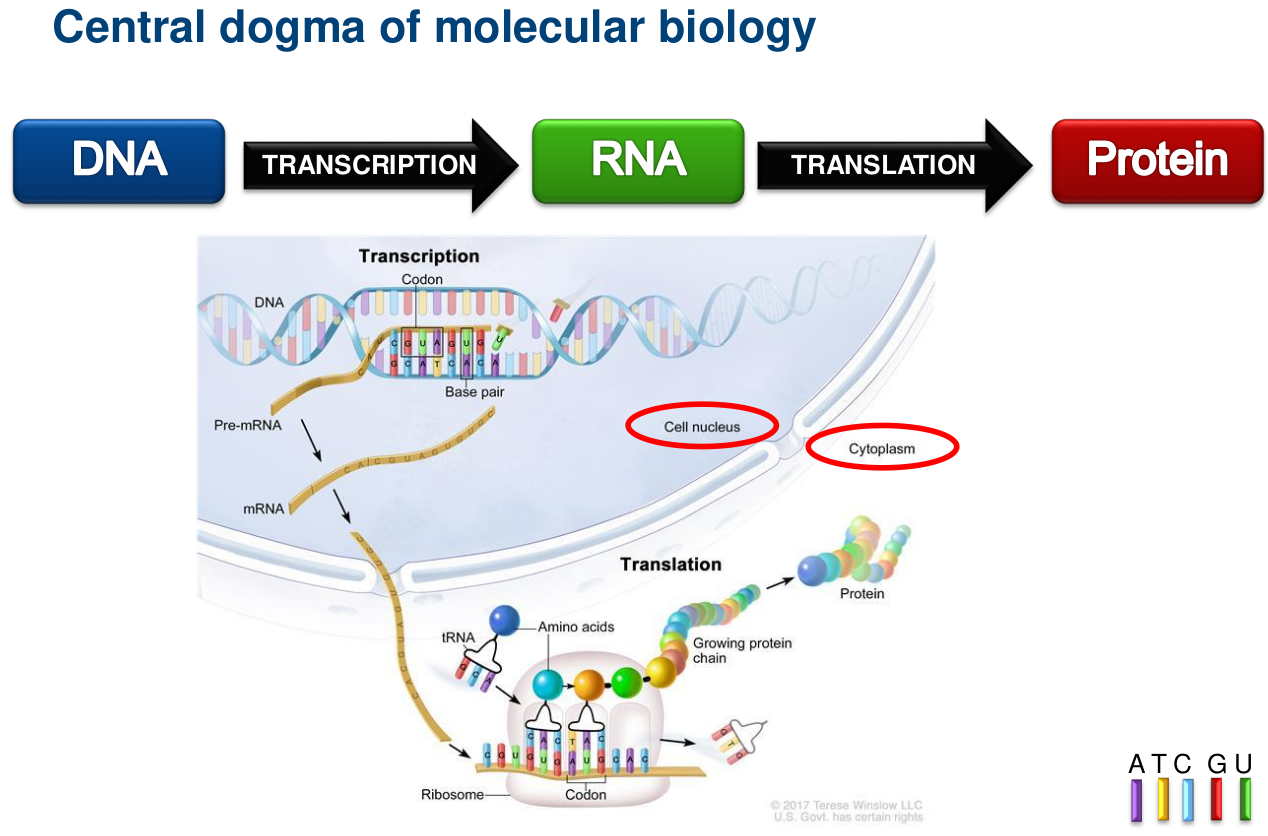
\includegraphics[width=0.9\linewidth]{figures/dogmaMolecularBiology.png}
	\caption{Protein biosynthesis \cite[p. 6]{schererStatisticalGeneticsGenetic2021}}
	\label{protein_biosynthesis}
\end{figure}

\begin{figure}[ht!]
	\centering
	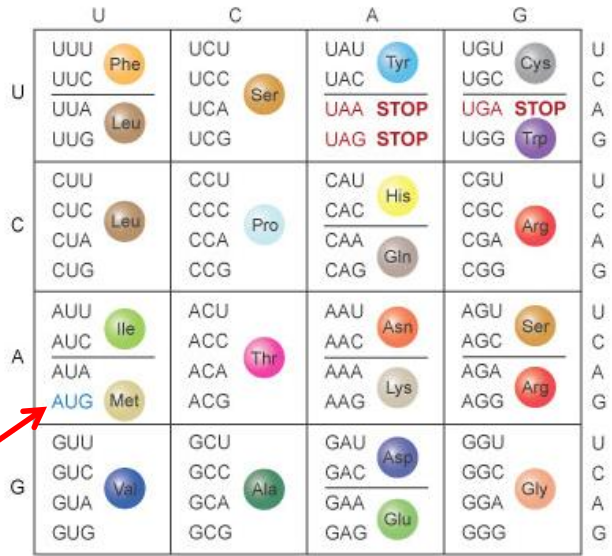
\includegraphics[width=0.5\linewidth]{figures/geneticCode.png}
	\caption{Genetic code \cite[p. 10]{schererStatisticalGeneticsGenetic2021}}
	\label{genetic_code}
\end{figure}


\subsubsection{Structure of \ac{SARS-CoV-2}} \label{fundamentalsAc}

\ac{RNA} based viruses (like \ac{SARS-CoV-2}) use \ac{RNA} to encode their genetic information. That means that the genetic information is present as a single strained \ac{RNA} sequence. This sequence contains for example the information on which proteins form the surface structure of the SARS-CoV-2 virus and how this surface looks like. \cite{NAQVI2020165878}

Based on Naqvi et al. \cite{NAQVI2020165878} the four proteins forming \ac{SARS-CoV-2} are:
\begin{itemize}
	\item spike (S)
	\item envelope (E)
	\item membrane (M)
	\item nucleocapsid (N)
\end{itemize}

A structural representation of \ac{SARS-CoV-2} and a host cell is visualized in \autoref{sarscov2_structure}. \cite{NAQVI2020165878}

\begin{figure}[ht]
	\centering
	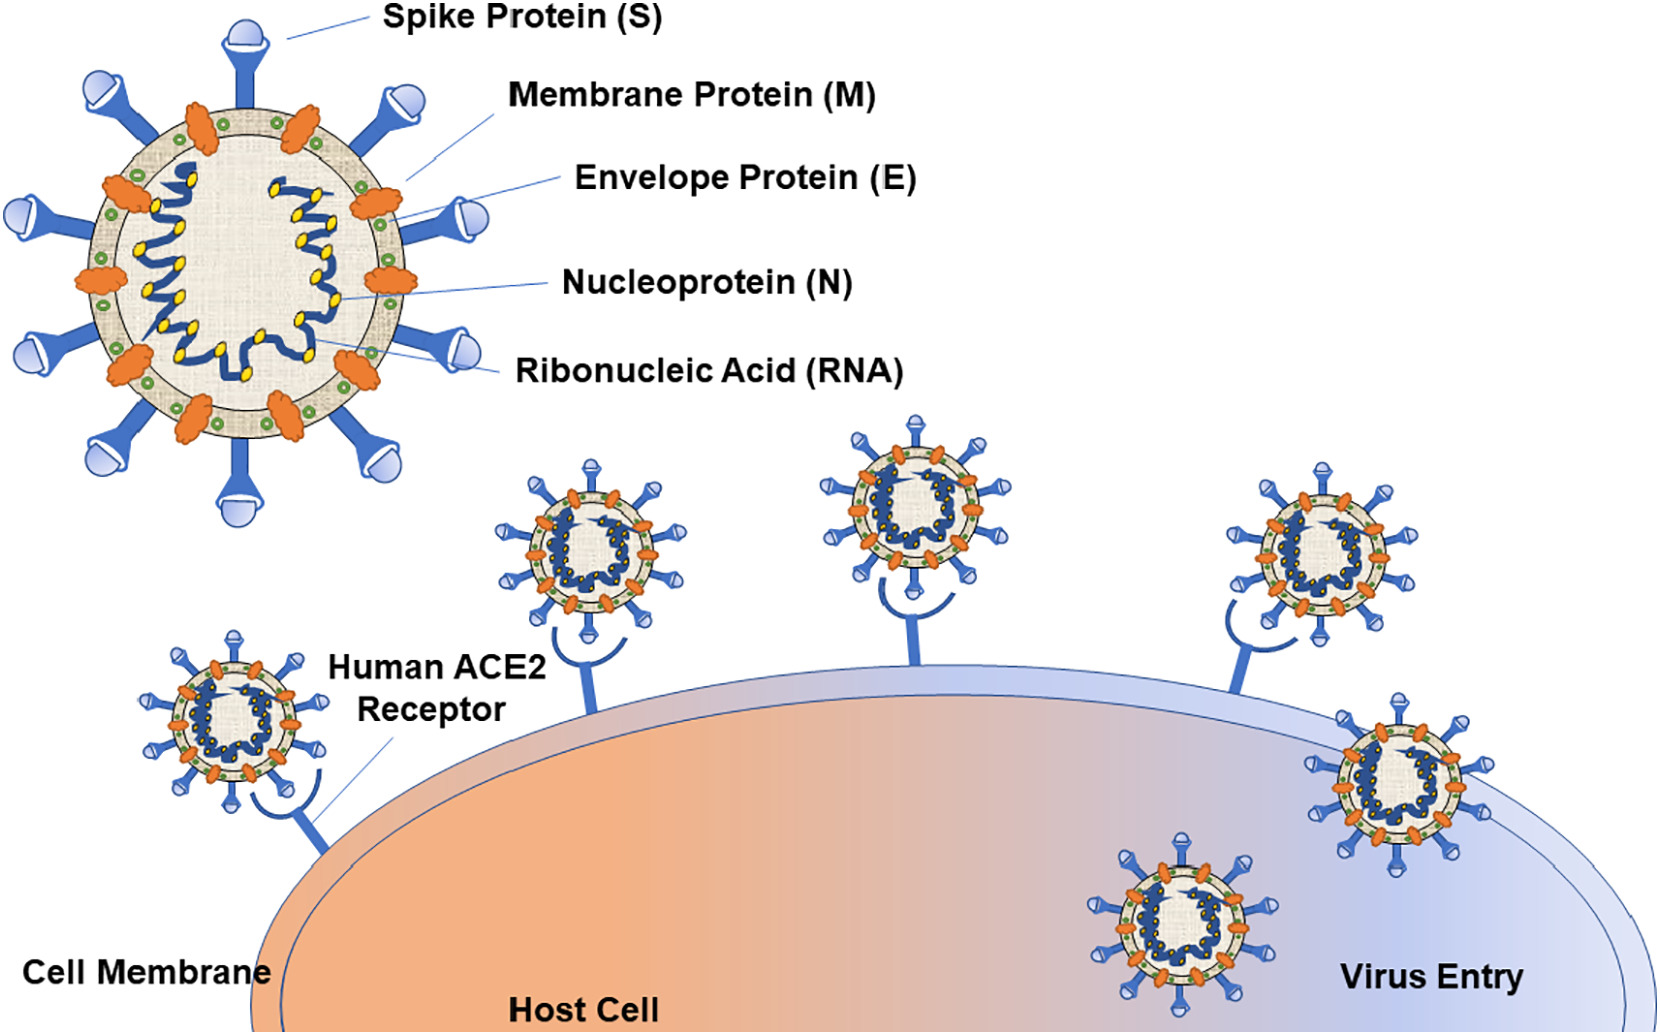
\includegraphics[width=0.8\linewidth]{figures/SARS-CoV-2Structure.jpg}
	\caption{SARS-CoV-2 structure \cite[p. 2]{NAQVI2020165878}}
	\label{sarscov2_structure}
\end{figure}

Furthermore \autoref{sarscov2_structure} shows the \ac{RNA} in the center. The \ac{SARS-CoV-2} \ac{RNA} consists of about 30,000 nucleotides, which belong to different subgroups, as shown in \autoref{sarscov2GenomeStructure}. 
Padded by a 5' \ac{UTR} at the beginning and a 3' \ac{UTR} in the end (\ac{UTR} are markers for the beginning and the end of protein-coding sequences), the middle part contains 12 functional \ac{ORF}, which contain the four coding regions for the proteins S, E, M and N. 

\begin{figure}[ht]
	\centering
	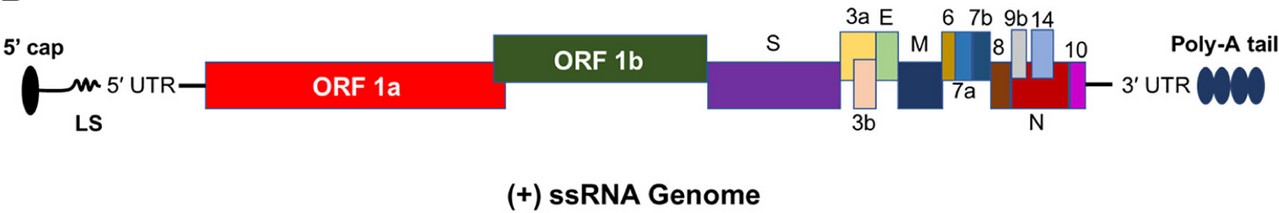
\includegraphics[width=1.0\linewidth]{figures/sarscov2GenomeStructure.png}
	\caption{\ac{SARS-CoV-2} genome structure \cite[p. 3]{NAQVI2020165878}}
	\label{sarscov2GenomeStructure}
\end{figure}

\subsubsection{Relationships between Biological Objects} \label{fundamentalsAd}

One main question in biology is to determine relationships between objects, such as species or genome sequences. The observed objects are called taxa. Most commonly used for determining these relationships is the phy\-lo\-ge\-ne\-tic analysis which generates a phy\-lo\-ge\-ne\-tic tree. In this phy\-lo\-ge\-ne\-tic tree, each leaf node corresponds to exactly one taxon. The inner nodes of the tree are the inferred hypothetical ancestors, which are no taxa. The relatedness between different taxa can be evaluated by their distance. \cite{böckenhauer2013algorithmische}

\autoref{examplePhylogeneticTree} shows an example phylogenetic tree calculated based on the species genomes. On the right side, each leaf node (taxa) corresponds to one current species. From left to right one can see the inferred historical development from the ancestors to the current species. One can see, that Gorillas and Orangutans have earlier developed apart than the other species. Furthermore one can see, that the  Chimpanzees and Bonobos share a most recent common ancestor (inner node next to both). That is why they are more related to each other. \cite{mallawaarachchiMolecularPhylogeneticsUsing2018}

\begin{figure}[ht]
	\centering
	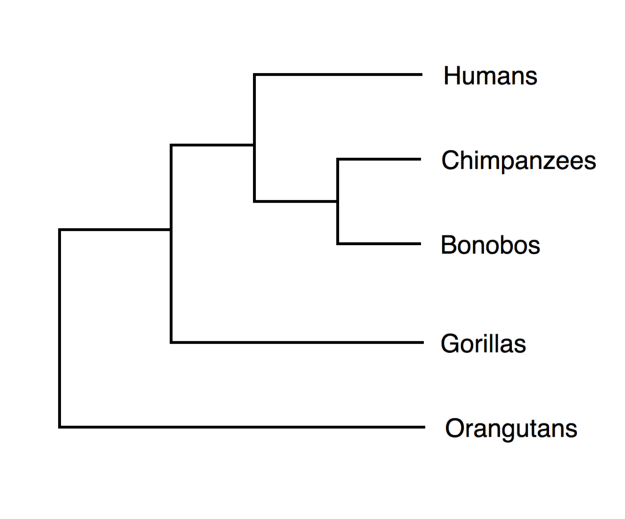
\includegraphics[width=0.5\linewidth]{figures/examplePhylogeneticTree.png}
	\caption{Example phylogenetic tree \cite{mallawaarachchiMolecularPhylogeneticsUsing2018}}
	\label{examplePhylogeneticTree}
\end{figure}

\newpage

\subsection{From Probabilistic Language Models to modeling Evolution Theory} \label{fundamentalsB}

A probabilistic language model tries to approximate the probability distribution 

\begin{equation}
	P(w_1, ..., w_n) = \Pi_{t=1}^{n} P(w_t | w_1, ..., w_{t-1})
\end{equation}

with $w_t$ being a word at position (time step) $t$ in a sentence of length $n$. To build language models \acp{RNN} were used to model such probability distributions. 

\begin{figure}[ht]
	\centering
	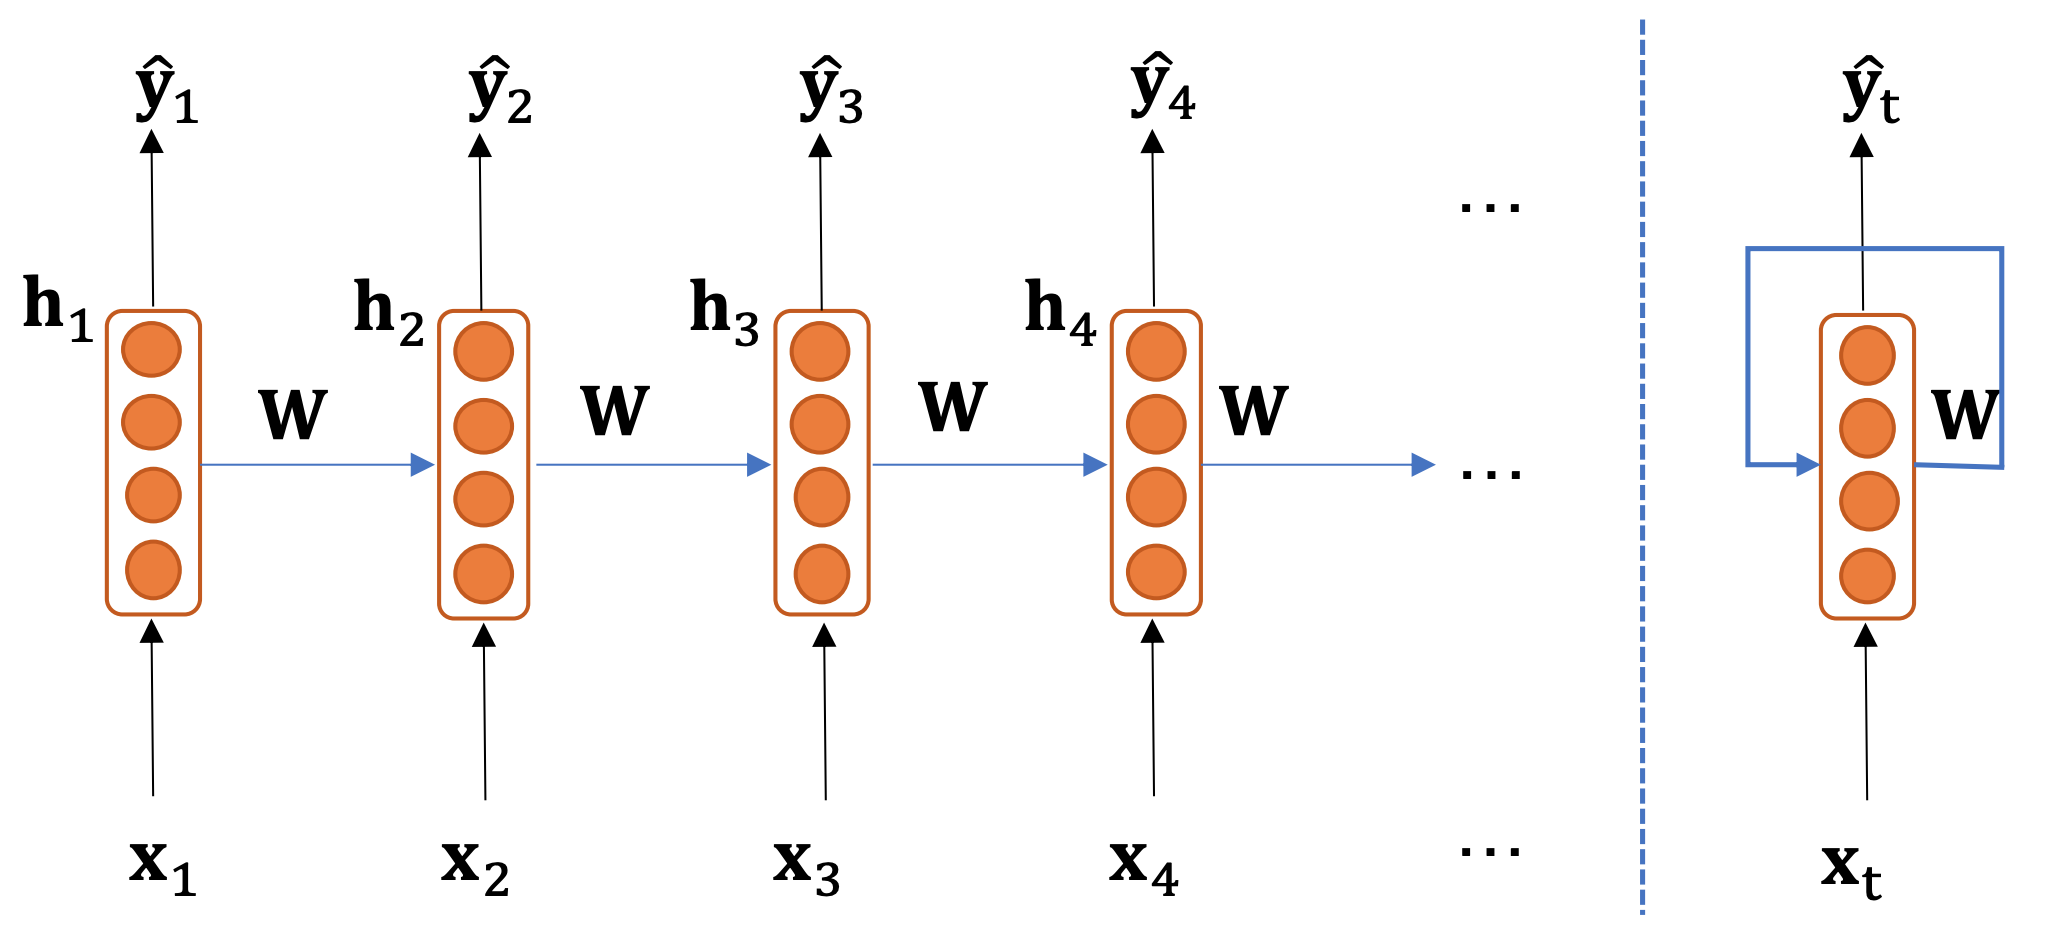
\includegraphics[width=0.6\linewidth]{figures/rnn_architecture.png}
	\caption{Architecture of a conventional \ac{RNN} \cite[p. 46]{Gertz2020}}
	\label{rnn_architecture}
\end{figure}

At each time step $t$ it outputs a probability distribution $P(w_t | w_1, ..., w_{t-1})$ given the words read so far in the current instance (see \autoref{rnn_architecture}). Words are read as a vectorized numerical representation, often given by pretrained so-called word embeddings $x_t$ which are lower-dimensional and more semantically enriched compared to simple one-hot encodings. One then calculates the hidden state $h_t$ by

\begin{equation}
	h_t = f(W^{(h)} h_{t-1} + W^{(x)} x_t + b_1)
\end{equation}

and the corresponding output probability distribution by 

\begin{equation}
	\hat{y}_t = softmax(U^{(h)} h_t + b_2).
\end{equation}

The applied weight matrix is always the same for each time step $t$ giving the \ac{RNN} its name. One can therefore simplify the unrolled \ac{RNN} architecture on the left side of \autoref{rnn_architecture} to the one on the right, where the hidden state is continuously passed as an input to the next time step. To achieve a better convergence behavior during training, one can also provide the expected hidden state of time step $t-1$ instead of using the predicted hidden state, which is called teacher forcing. \acp{RNN} can process input of arbitrary length and are by their recurrent character capable to use information from previous time steps. Unfortunately, they are vulnerable to vanishing and exploding gradient problems. \ac{LSTM} is a special \ac{RNN} architecture that solves such vulnerabilities by owning a separate long-term cell state besides a short-term hidden state (introduced in \autoref{fundamentalsF}). It can preserve information over many time steps. \cite{Gertz2020}

\begin{figure}[ht]
	\centering
	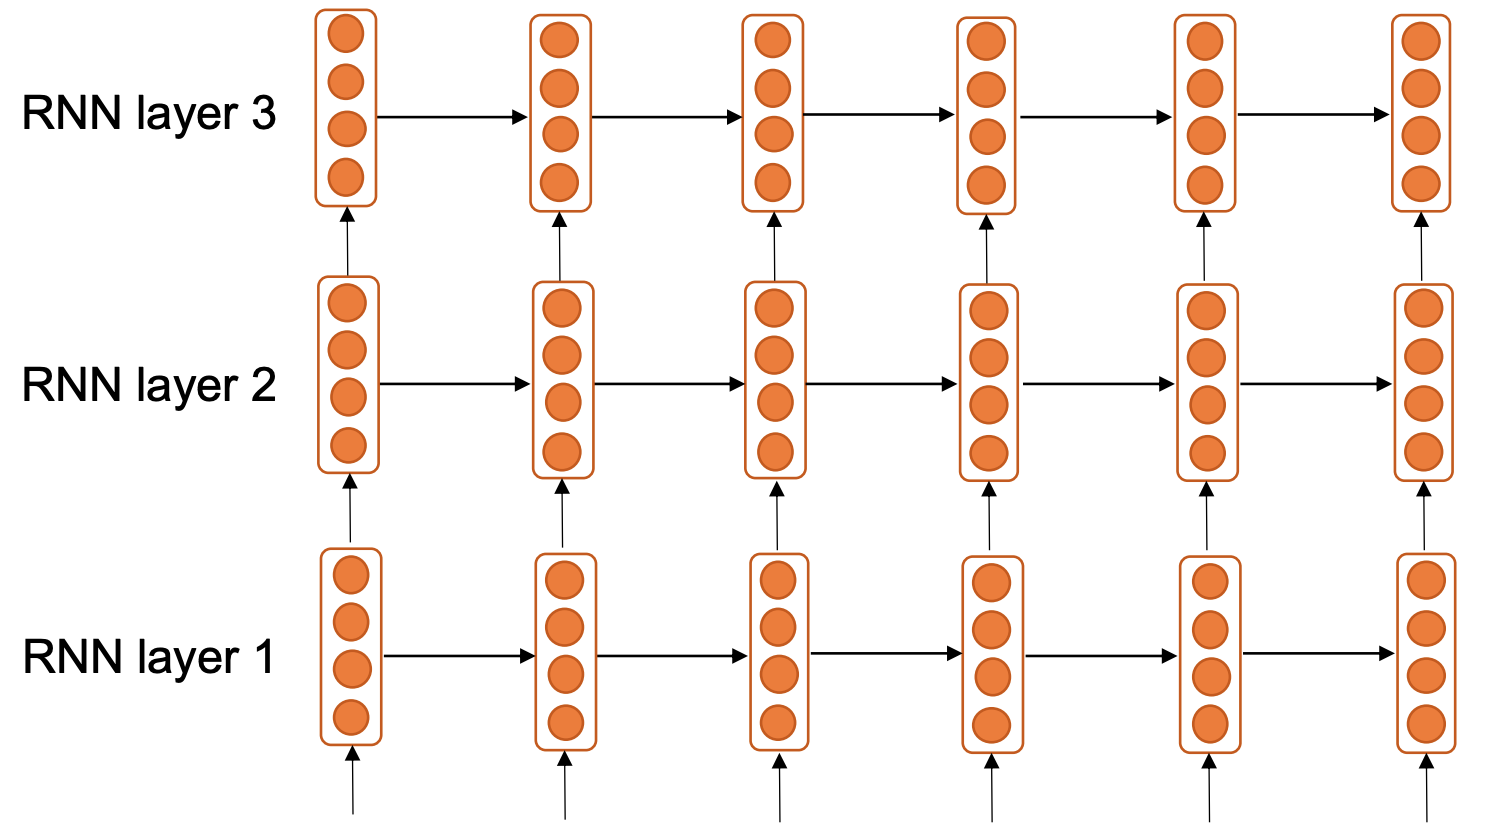
\includegraphics[width=0.6\linewidth]{figures/multi_layer_rnn.png}
	\caption{Architecture of a multi-layer  \ac{RNN} \cite[p. 87]{Gertz2020}}
	\label{multi_layer_rnn}
\end{figure}

One can also use two \acp{RNN}, one traversing a sentence from left to right and another one vice versa, with two different weight matrices to model the probability distribution bidirectionally. One therefore simply concatenates the hidden states of each \ac{RNN} before applying the weight matrix $U$ and the $softmax()$ function. Also multi-layer \acs{RNN} can be utilized to generate higher-order features (hidden states) for the prediction task (see \autoref{multi_layer_rnn}). \cite{Gertz2020}

The \acp{RNN} or even better \acp{LSTM} architectures used for probabilistic language modeling can be reused in a more complex domain called sequence to sequence modeling for \ac{NMT} from one language to another. Here one first tries to learn a fixed-dimensional input representation from an input sequence using an encoder architecture based on an \ac{LSTM}. The so-called context vector is then decoded by a second \ac{LSTM} into a new sequence of words preserving the grammar but having a different meaning. \cite{Sutskever2014}

Sequence to sequence models are introduced together with the \ac{LSTM} architecture in \autoref{fundamentalsF}. Here the connection to evolution theory can be drawn. \ac{RNA} sequences made of a concatenation of nucleotides \footnote{We restrict the representation of nucleotides solely to their nucleobases parts consisting of the distinct nucleobases guanine, adenine, cytosine and thymine. We therefore do not include the phosphate group and the five-carbon sugar components.} can be represented textually using the FASTA format \cite{cockBiopythonFreelyAvailable2009}. A \ac{Seq2Seq} model can then transferable be applied in the domain of \ac{RNA} sequences to model how \ac{RNA}-based viruses change their structure to avoid the detection by the human immune system but still to preserve their infectivity and evolutionary fitness \cite{Hie2021}. 

\subsection{GISAID EpiFlu Data Platform} \label{fundamentalsC}

The data needed for this project consists of the \ac{SARS-CoV-2} genome data and the corresponding metadata. The most complete database is hosted by the \ac{GISAID} initiative \cite{Gisaid2021}. It is a public-private partnership between the initiative itself and the governments of Germany (official host of the platform), Singapore and the United States of America. \cite{gisaideditorGISAID2021}

The main aim of \ac{GISAID} is to enable the fast sharing of epidemic and pandemic virus data. In comparison to other databases such as GenBank the genome sequences are shared fast through \ac{GISAID}. For enabling this fast sharing the \ac{GISAID} database is only usable after registration and the redistribution of the data is forbidden, whereas the GenBank database is publicly available. \cite{shuGISAIDGlobalInitiative2017}

Thus, until september 2021 over three million \ac{SARS-CoV-2} genome sequences are available through \ac{GISAID}, whereas only about one million \ac{SARS-CoV-2} genome sequences are available through GenBank. \autoref{gisaid} shows the selection view of the \ac{GISAID} database. \cite{gisaideditorGISAID2021, nationallibraryofmedicinencbieditorNCBISARSCoV2Resources}

\begin{figure}[ht]
	\centering
	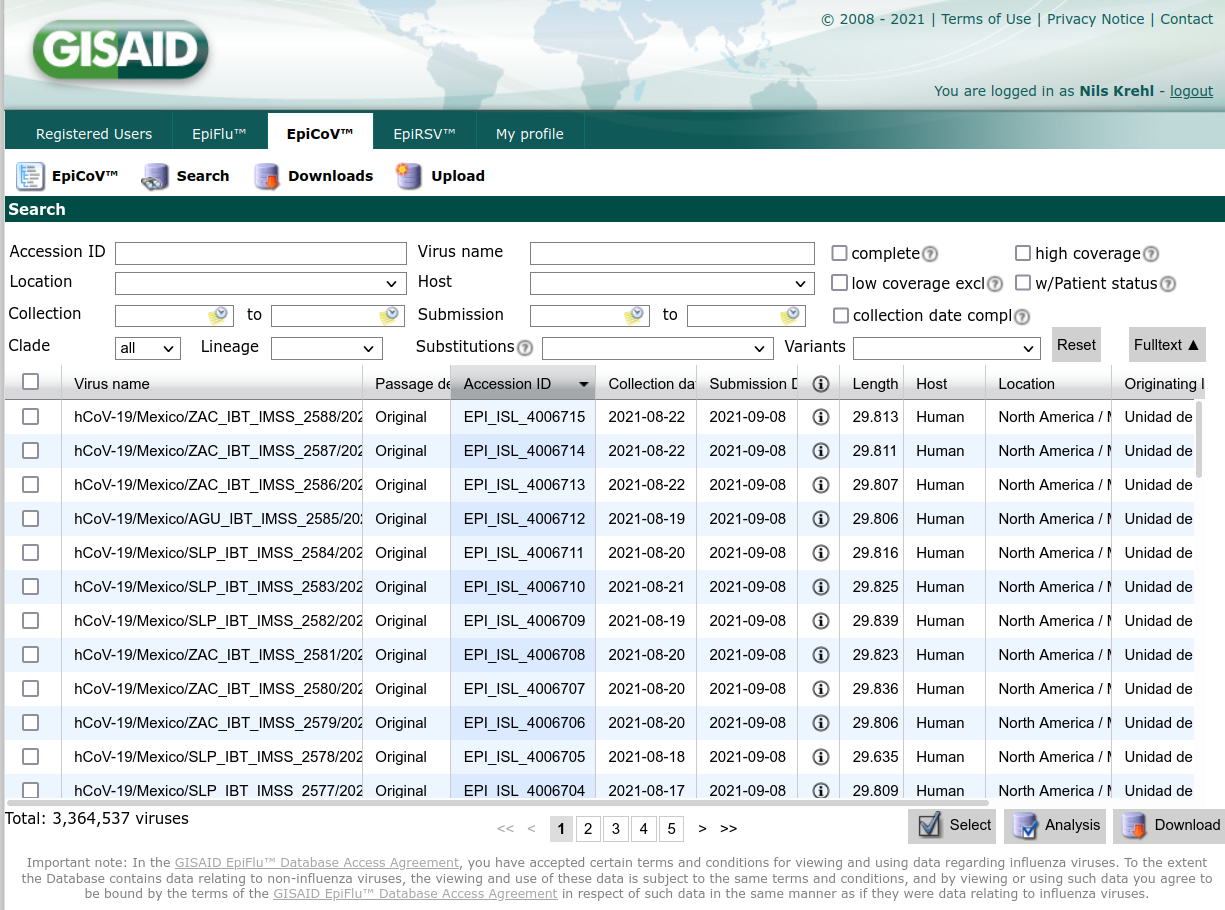
\includegraphics[width=0.9\linewidth]{figures/gisaid.png}
	\caption{\ac{GISAID} database \cite{own screenshot}}
	\label{gisaid}
\end{figure}


\subsection{Domain-Specific Methodologies to create Evo\-lu\-tio\-na\-ry Datasets for Mutation Prediction} \label{fundamentalsD}

From databases such as \ac{GISAID} or GenBank an unordered list of genome sequences and metadata can be downloaded. For training a \ac{ML} model to detect changes and predict future mutations the dataset must contain parent-child pairs.

Berman et al. \cite{Berman2020} have done this based on two steps. First, they created a phylogenetic tree from the genome sequences. Therefore first all genome sequences are aligned. The initial phylogenetic tree is calculated by Fasttree using the approximate maximum likelihood method. In the next step, the tree is refined by a generalized time-reversible (GTR) model and a gamma model. The final phylogenetic tree is achieved by optimizing the branch length and the used models for tree generation. Like in standard phylogenetic trees each leaf node corresponds to one data instance, whereas the inner nodes are inferred from the other data instances.
Secondly based on the rooted phylogenetic tree, parent-child pairs are calculated. Therefore first a marginal ancestral sequence reconstruction is executed based on the phylogenetic tree from the previous step. Now also the inner nodes correspond to data instances. In the next step BioPython's \cite{10.1093/bioinformatics/btp163} Bio.Phylo package is used to determine parent-child pairs. From each edge, one parent-child pair is generated. \cite{Berman2020}

Mohamed et al. \cite{Mohamed2021} used existing datasets from Ogali et al. \cite{ogaliMolecularCharacterizationNewcastle2018} in their work about mutation prediction. Ogali et al. \cite{ogaliMolecularCharacterizationNewcastle2018} performed a phylogenetic analysis. After selecting only genome sequences with high quality, they removed duplicate sequences and added reference sequences to the dataset. Now the alignment is executed. In the next step MEGA (Molecular Evo\-lu\-tio\-na\-ry Genetics Analysis) is used to create the phylogenetic tree. This is done by using the maximum likelihood method, the best-fit general time-reversible (GTR) model and gamma-distributed rate variation.

Hadfield et al. \cite{10.1093/bioinformatics/bty407} have created the nextstrain project. It aims to examine pathogen's spread and evolution by providing a viral genome database, a bioinformatics pipeline for phylodynamics analysis and a visualization plat\-form. Steps executed by the bioinformatics pipeline for phylodynamic analysis are: "subsampling, alignment, phylogenetic inference, temporal dating of ancestral nodes and discrete trait geographic reconstruction, including in\-fe\-rence of the most likely transmission events" \cite{10.1093/bioinformatics/bty407}. For calculating the phylogenetic tree, TreeTime's maximum likelihood method is used. \cite{10.1093/bioinformatics/bty407}

\subsection{Previous Work on Mutation Prediction} \label{fundamentalsE}

Even before the rise of Covid-19, there had been studies trying to predict mutations of \ac{RNA} viruses. In the collection of \cite{Yan2007, Wu2007, Wu2008} the authors predict the mutation positions in hemagglutinins from influenza A virus using logistic regression and plain neural networks and then use the resulting amino acid mutating probabilities to derive possible mutated amino acids. The same approach is further used for H5N1 neuraminidase proteins. 

Salama et al. \cite{Salama2016} proved that nucleotides in an \ac{RNA} sequence can change based on their local neighborhood. Neural networks are used to predict new strains of the Newcastle virus and subsequently, a rough-set theory based algorithm is introduced to extract the according point mutation patterns. 

Mohamed et al. \cite{Mohamed2021} used a more modern sequence to sequence approach based on \acp{LSTM} to learn nucleotide mutations between time-series species of H1N1 Influenza virus and the Newcastle virus as mutations can also be influenced by long-distance relations of amino acids. Therefore one-hot-encoded \ac{RNA} sequences of a parent generation preprocessed to words are given as an input and the output is the predicted offspring generation evaluated by accuracy to the compared true offspring generation. The achieved accuracy in this paper is questionably high with 98.9\% on the H1N1 Influenza virus and 96.9\% on the Newcastle virus, possibly because of overfitting to the few 4.609 samples for H1N1 Influenza virus and only 83 for the Newcastle virus. The approach in this paper therefore tries to increase the number of samples available for training when building the dataset. 

\vspace{0.5cm}
The approach in this paper will neither use any of the just mentioned architectures but uses a transformer-based architecture coupled with a \ac{GAN}-style training architecture. A short introduction into \ac{Seq2Seq} models and the underlying \ac{LSTM} components shall be given to better point out the architectural decisions made. 

\subsection{Sequence-to-Sequence Models based on Long Short-Term Memory} \label{fundamentalsF}

The original \ac{LSTM} unit was introduced by Hochreiter and Schmidhuber in \cite{Hochreiter1997} and can be used for language modeling instead of using plain \acp{RNN} to prevent running into vanishing or exploding gradient problems \cite{Sundermeyer2012}. The architecture of an \ac{LSTM} is shown in \autoref{lstm_architecture}.

\begin{figure}[ht]
	\centering
	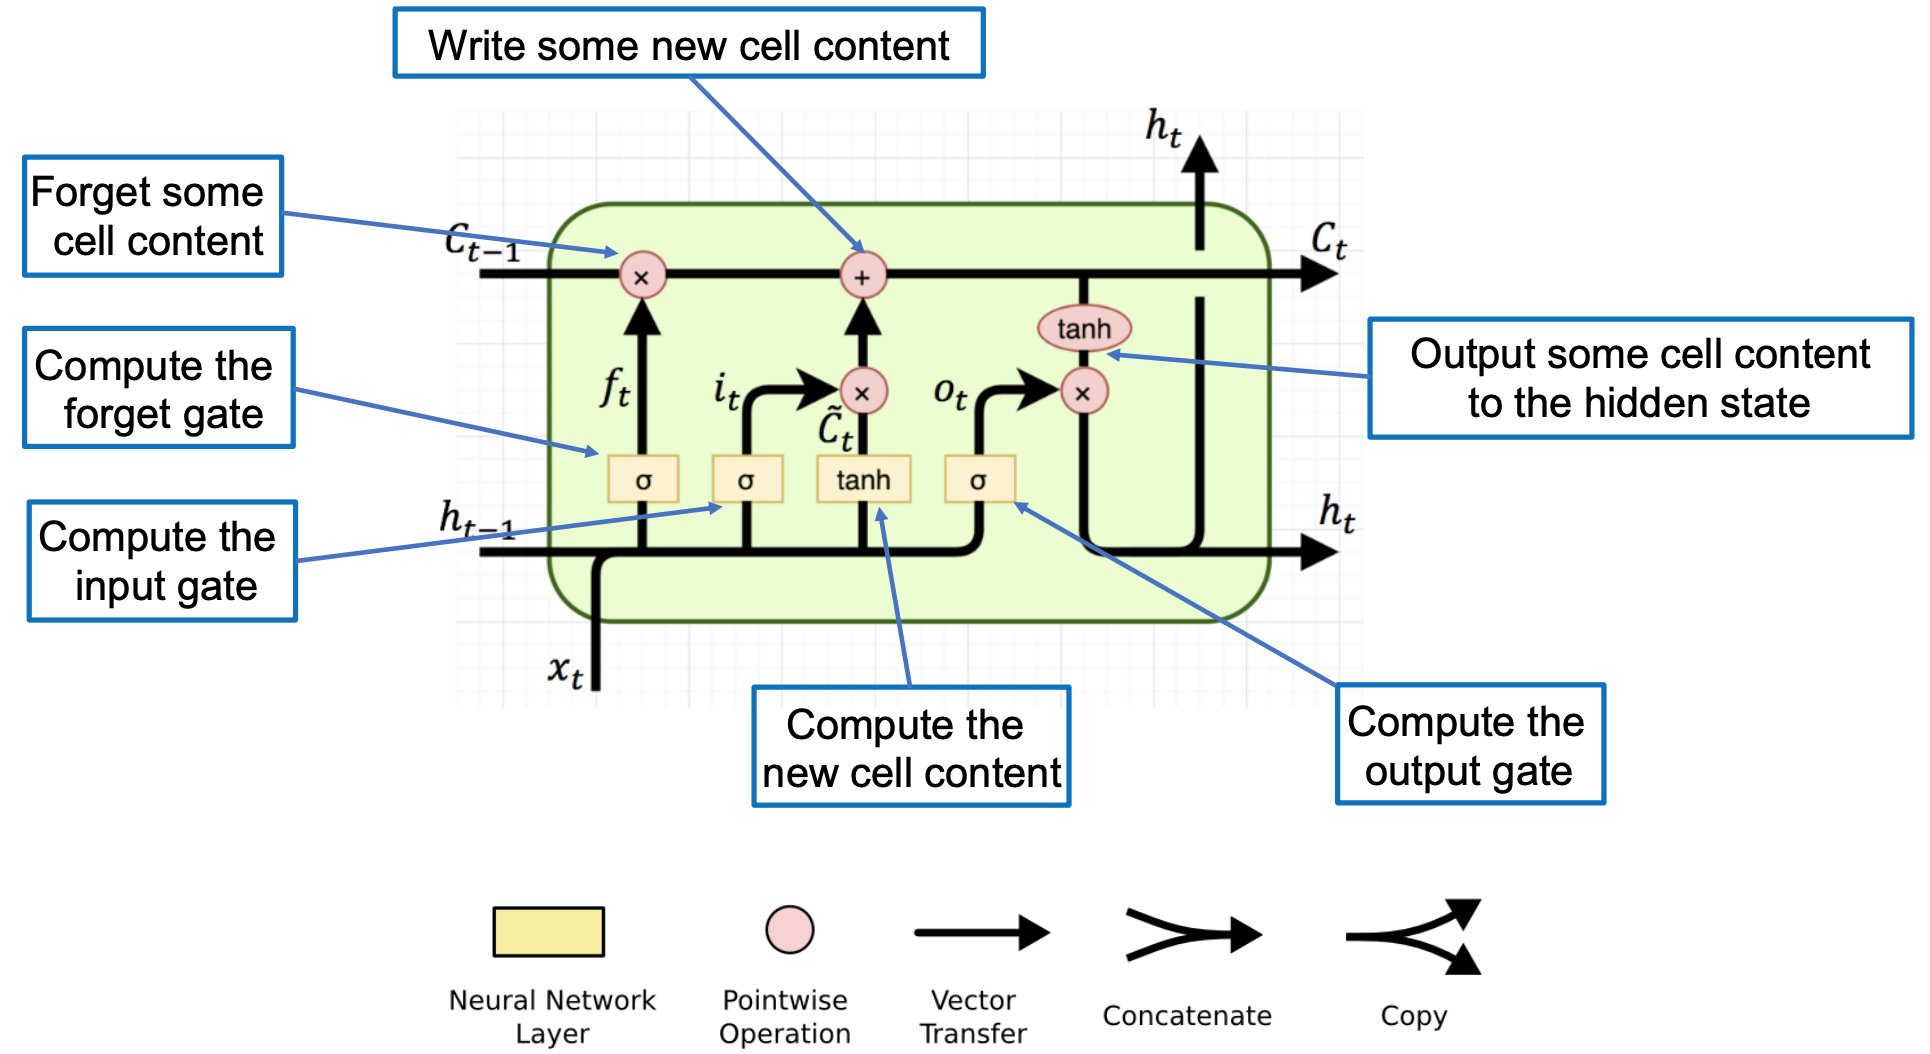
\includegraphics[width=\linewidth]{figures/lstm_architecture.png}
	\caption{Architecture of an \ac{LSTM} \cite{Gertz2020}}
	\label{lstm_architecture}
\end{figure}

It consists of a hidden state $h_t$ and an additional cell state $c_t$. The cell state stores long-term information and is used to derive a new hidden state. Information flows through three different gates inside the \ac{LSTM}. The forget gate is used to control which parts of the cell state are potentially carried on to the next time step, the input gate is responsible to decide which parts of the cell state should be updated and the output gate determines what is being passed on as the new hidden state. All three gates depend on the previous hidden state and the current input. They provide factors limited to the interval [0,1] by the sigmoid function and are multiplied with the cell state, the changes to be added to the cell state and the new hidden state derived from the cell state. Through the cell state, an \ac{LSTM} therefore makes it possible to capture long-distance dependencies. \cite{Gertz2020}

Sutskever et al. \cite{Sutskever2014} introduced \ac{Seq2Seq} learning following a multi-layer encoder-decoder style model architecture. One layer consists of one \ac{LSTM} that is used as an encoder to learn a large fixed-dimensional vector representation of a size-unrestricted input sequence called the context vector. This vector consists of the last cell and hidden state of the encoder and incorporates the structure of the input sequence helping the following decoder \ac{LSTM} to provide qualitative predictions for the output sequence. The second \ac{LSTM} therefore serves as a beam search\footnote{Do not choose the most probable word but the $B$ most likely word hypothesis and pass them to the next time step in the \ac{LSTM}. Whichever hypothesis results in the lowest loss is kept. To avoid combinatorial explosion limit the beam depth size.} decoder to map the context vector to a corresponding output sequence whose length does not need to match with the length of the input sequence. The output probability distribution is therefore given by the equation

\begin{equation}
	p(y_1, ..., y_{T'} | x_1, ..., x_{T}) = \Pi_{t=1}^{T'} p(y_t | v, y_1, ..., y_{t-1})
\end{equation}

with $v$ being the context vector. Using an \ac{LSTM} is preferred over a normal \ac{RNN} as it is used to capture the long-range temporal dependencies of the input data. The encoder-decoder architecture uses four layers in total partitioned onto four \acp{GPU}. A corpus of 160k words for the input sequence and another one of 80k words for the target sequence was used to create the word embeddings of dimension 1000. Unknown words were replaced by an \textit{UNK} token. The \ac{Seq2Seq} model approach was evaluated for \ac{NMT} and reached a 34.81 \ac{BLEU} score. One finding during training was that reversing the input sequence introduces many short-term dependencies as the minimal time lag of the problem is reduced making optimization easier. \cite{Sutskever2014}

\subsection{Applying Generative Adversarial Networks} \label{fundamentalsG}

Using a plain \ac{Seq2Seq} model for mutation prediction does not necessarily guarantee that the generated sequences are evolutionary offsprings of a parent generation as not being included as is in the ground truth data. The generated sequences might occur realistic and biologically relevant, but a plain sequence to sequence architecture does not inherently check for natural parental descent and therefore does not make sure whether the predicted mutations lead to improved fitness. Berman et al. \cite{Berman2020} developed a novel \ac{Seq2Seq} framework based on the \ac{GAN} idea to predict genetic mutations and future biological populations of the influenza virus (see \autoref{mutagan}). Muta\-GAN describes a \ac{Seq2Seq} generator within an adversarial framework that predicts protein sequences augmented with possible mutations. By using a \ac{Seq2Seq} generator and a discriminator specialized on separating fake evolutionary mutations from real ones, one can then guarantee to a certain degree that the evolutionary parent-childhood coherence is given. In MutaGAN a mutation is considered correct if the change in amino acid and location within the \ac{RNA} sequence is equal to the parent's true offspring. \cite{Berman2020}

\begin{figure}[ht]
	\centering
	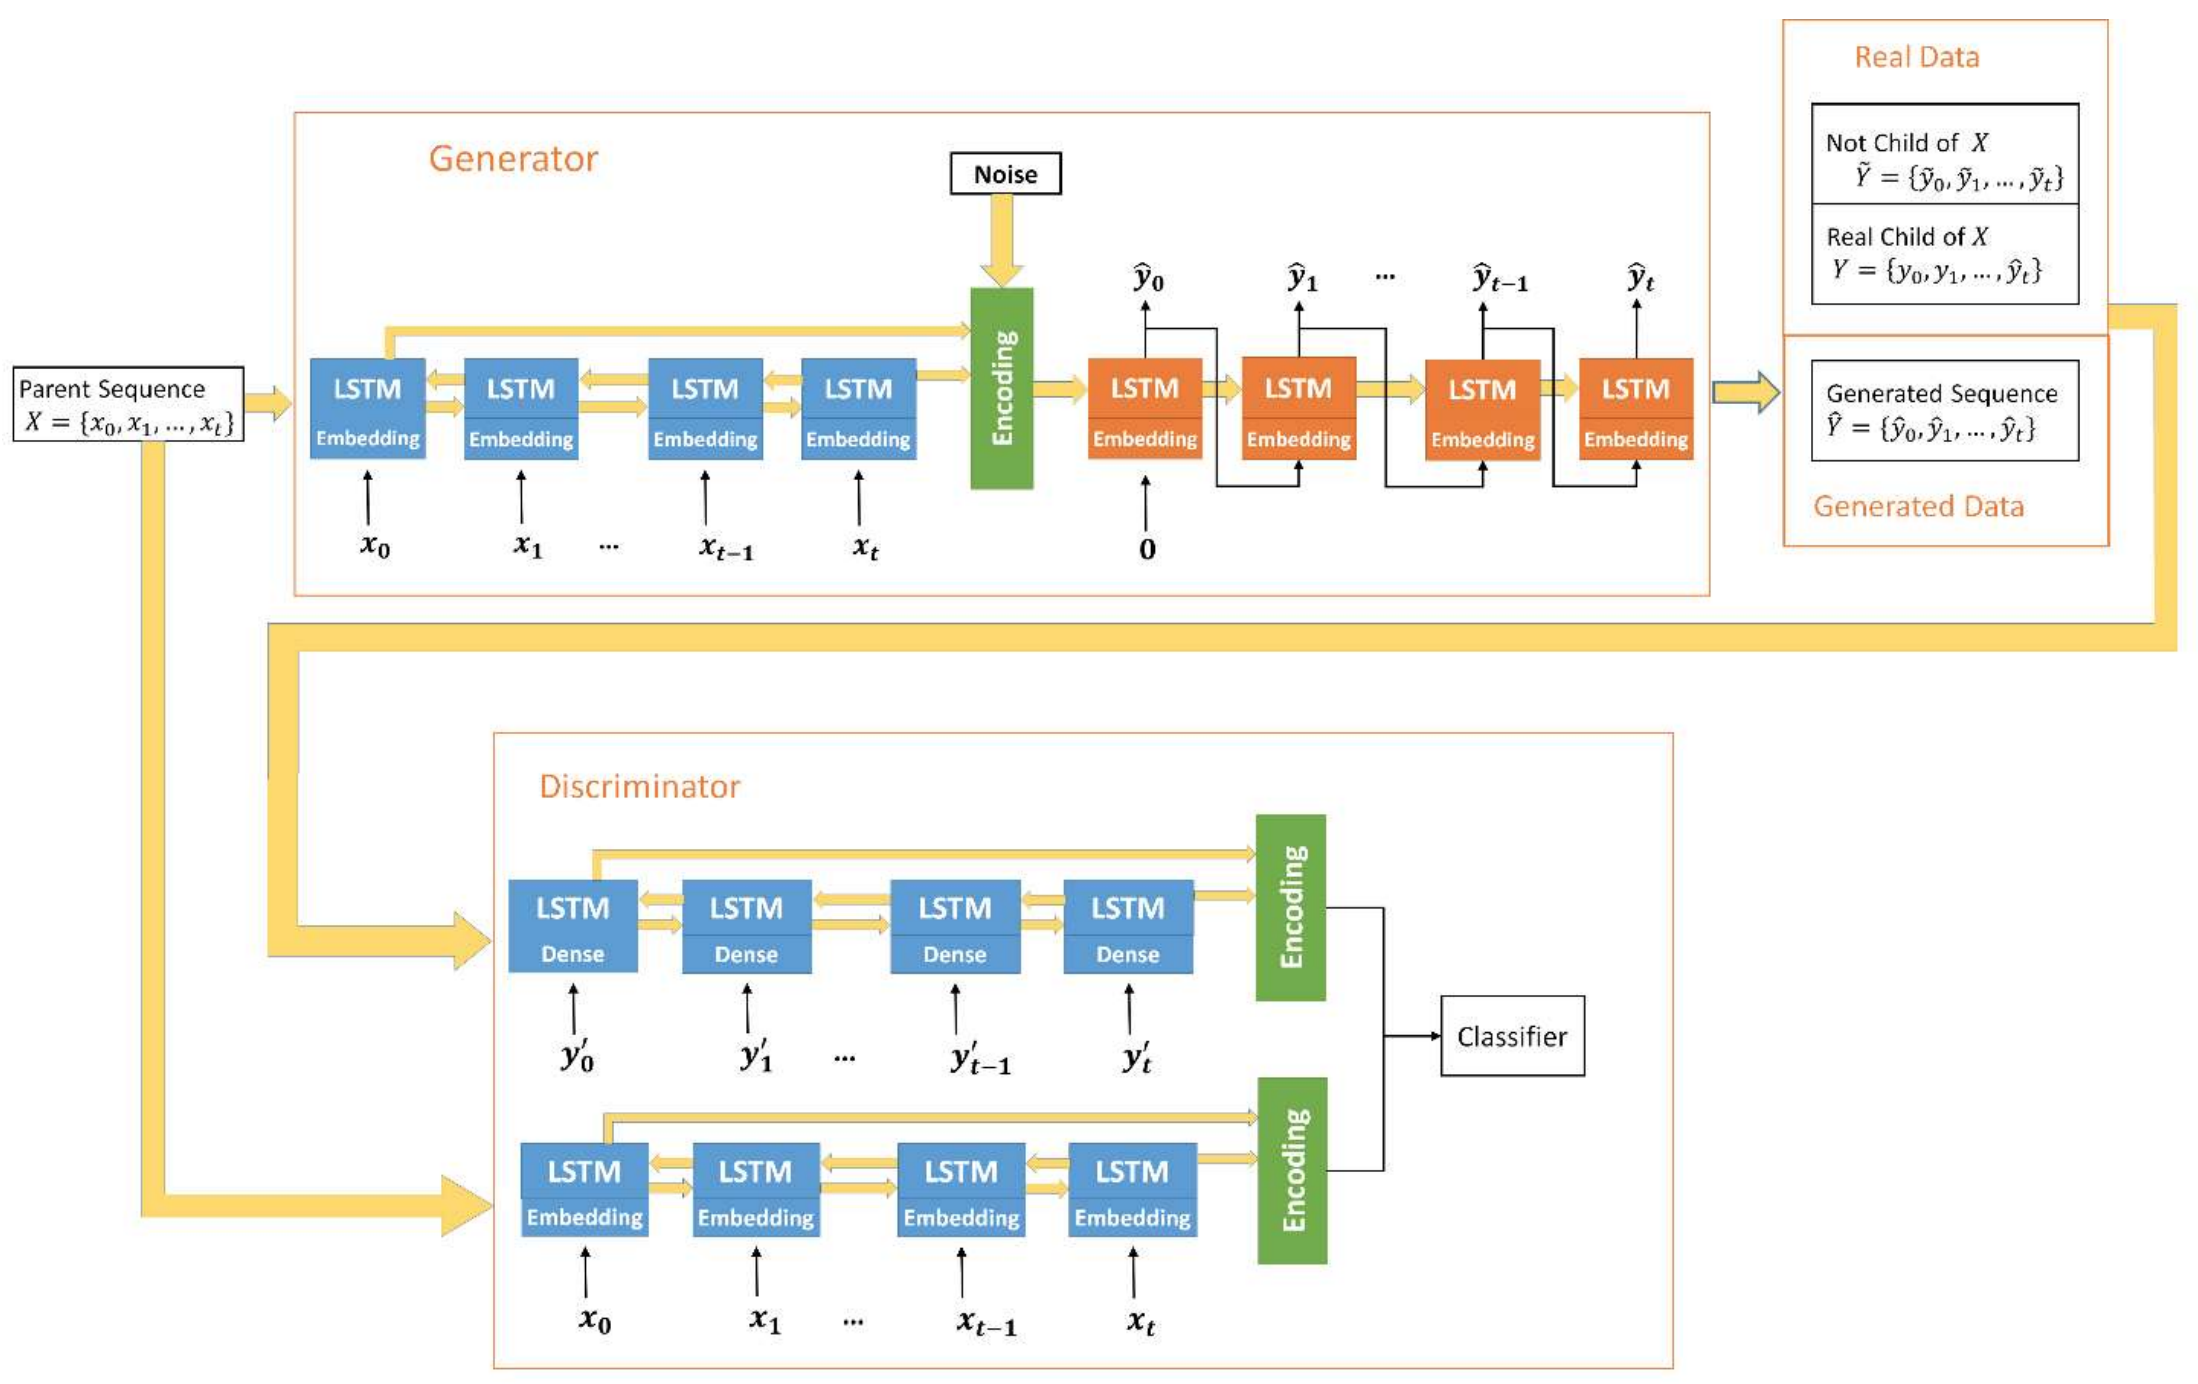
\includegraphics[width=\linewidth]{figures/mutagan.png}
	\caption{Architecture of MutaGAN \cite{Berman2020}}
	\label{mutagan}
\end{figure}

MutaGAN's generator consists of a \ac{Seq2Seq} model. The encoder is built of a bidirectional \ac{LSTM} and the resulting context vector of dimensionality 512 is combined with noise from a standard normal dis\-tri\-bu\-ti\-on. The decoder \ac{LSTM} predicts the resulting sequence of amino acids greedily using the $argmax()$ of the $softmax()$ output for every time step. The discriminator is trained on three different parent-child pair configurations to optimally compete against the generator, real parent-child pairs, real parent and generated child pairs and pairs of real sequences that are not parent-child pairs. Two bidirectional \ac{LSTM} encoders sharing the same weight matrix as the encoder of the generator produce a fixed-dimensional encoding of the provided parent-child pair used for classification of evolutionary descent by a plain neural network. The child encoder in the discriminator uses a dense layer having the same weight matrix as the embedding layer of the encoder of the generator. The dense layer is required to directly input the predicted child sequence as its probability distribution rather than the final output after applying the $argmax()$ as it would not enable backpropagation to train the generator. When a true child sequence is given a simple one-hot encoding is used. \cite{Berman2020}

Interestingly Berman et al. \cite{Berman2020} state planned improvements by utilizing bigger datasets acquired from the \ac{GISAID} database EpiFlu and by using more length-robust attention-based models to directly work on nucleotide sequences instead of sequences of amino acids. Therefore transformers and the attention mechanism are introduced in the following section.

\subsection{Transformer and Attention Mechanism} \label{fundamentalsH}

Using a \ac{Seq2Seq} model as introduced based on an encoder-decoder architecture of \ac{LSTM} cells has some drawbacks. First, the input needs to be processed sequentially in time steps which makes parallelization difficult and increases training time, especially for longer sequences. Fur\-ther\-mo\-re, the hidden and cell state vector passed through every timestep tries to encode information of \textit{all} previous time steps without knowing which information is especially important for the current time step. This not only makes long-distance dependencies hard to capture but also might not get the prioritization of the previous time step inputs right. \cite{Bahdanau2016, Vaswani2017} 

To tackle these problems the so-called transformer architecture was in\-tro\-du\-ced in \cite{Vaswani2017}. It feeds an entire sequence into the encoder to be processed in parallel denying any concept of recurrence or convolution. Only using a so-called self-attention mechanism the transformer makes sure that during processing every input position, receives the information that is most important to it. This way modeling long dependencies becomes much easier compared to \acp{LSTM} as the view on the input sequence is more global. In this architecture, the encoder also passes all computed hidden states of every position to the decoder, which therefore can generate the target sequences based on more semantically enriched features and also in parallel for every position. \cite{Vaswani2017}

The transformer architecture achieved state-of-the-art quality results with a \ac{BLEU} score of 41.8 on the WMT 2014 English-to-French translation task (cf. \ac{BLEU} score of \cite{Sutskever2014} was 34.8), while still being much faster to train due to its parallelization capabilities. State-of-the-art results are already achieved after just twelve hours of training on eight P100 \acp{GPU}. As this is still far beyond the scope and resources given for this project, this project provides a proof-of-concept transformer model trained for far shorter and fewer sequences as one would need to predict entirely new \ac{RNA} sequences. \cite{Vaswani2017}

First the transformer architecture should be introduced in the following:

\begin{figure}[ht]
	\centering
	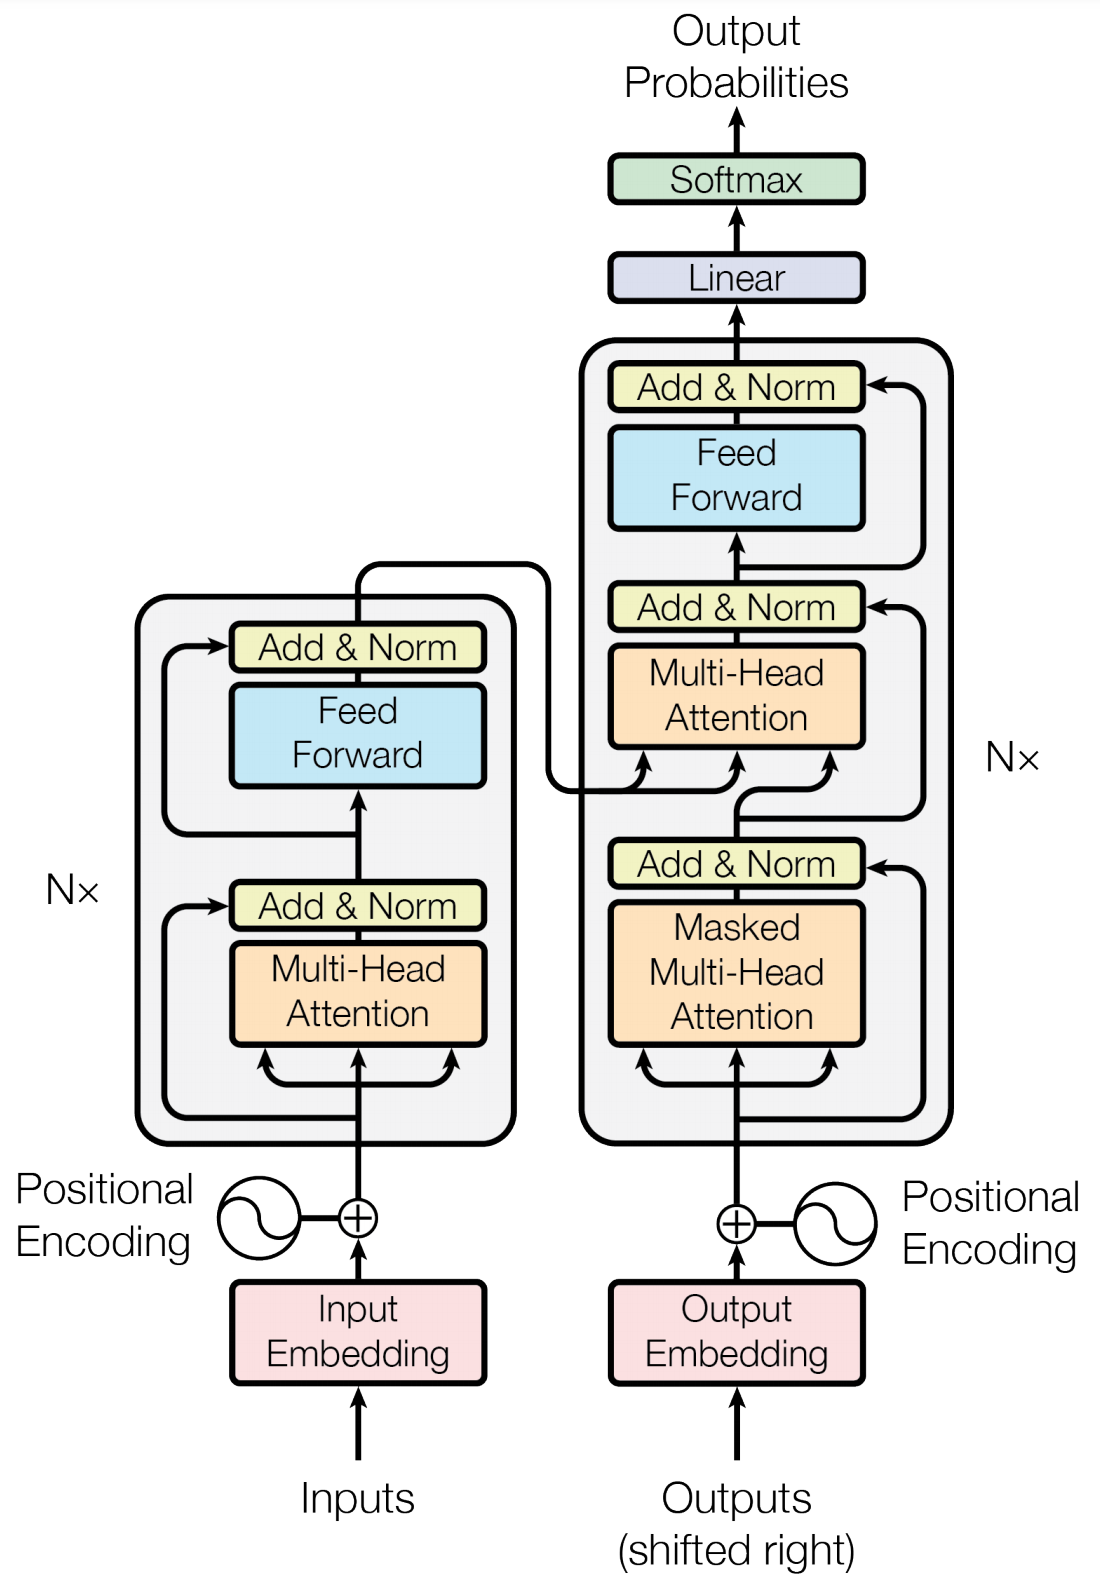
\includegraphics[width=0.5\linewidth]{figures/transformer.png}
	\caption{Architecture of the transformer \cite{Vaswani2017}}
	\label{transformer}
\end{figure}

The transformer consists of an encoder and a decoder part just as normal \ac{Seq2Seq} models. One layer of the encoder contains a self-attention layer before passing the hidden state representations of an input sequence to a feed-forward neural network consisting of two linear trans\-for\-ma\-ti\-ons separated by \ac{ReLU}. Thus it makes sure that semantic and contextual dependencies between different positions in the input sequence are also modeled. Also, skip connections are added for both components with subsequent layer normalization. \cite{Alammar2018, Vaswani2017}

To calculate the self-attention output of a sequence, a query $Q$, key $K$ and value $V$ matrix is calculated through the multiplication of the sequence representation\footnote{A matrix containing the hidden state representations of every input position} with learned transformation matrices. Each row of the three received matrices corresponds to a specific input position. The output of the self-attention layer is then calculated through

\begin{equation}
	(Scaled Dot-Product) Attention(Q, K, V) = softmax(\frac{QK^T}{\sqrt{d_k}})V.
\end{equation}

The dot product between $Q$ and $K$ calculates scores that are used as weighting factors for $V$. This describes for every input position how relevant all other input positions are for each of the hidden state encodings. The scores are divided by the square root of the dimensionality of the query/key values of the hidden state representations, which is chosen to be 64 (square root eight), to receive more stable non-vanishing gradients. The softmax guarantees that the positional scores lie between zero and one and add up to one. Note that the score of the current input position itself will most likely have the highest score. \cite{Alammar2018, Vaswani2017}

\begin{figure}[ht]
	\centering
	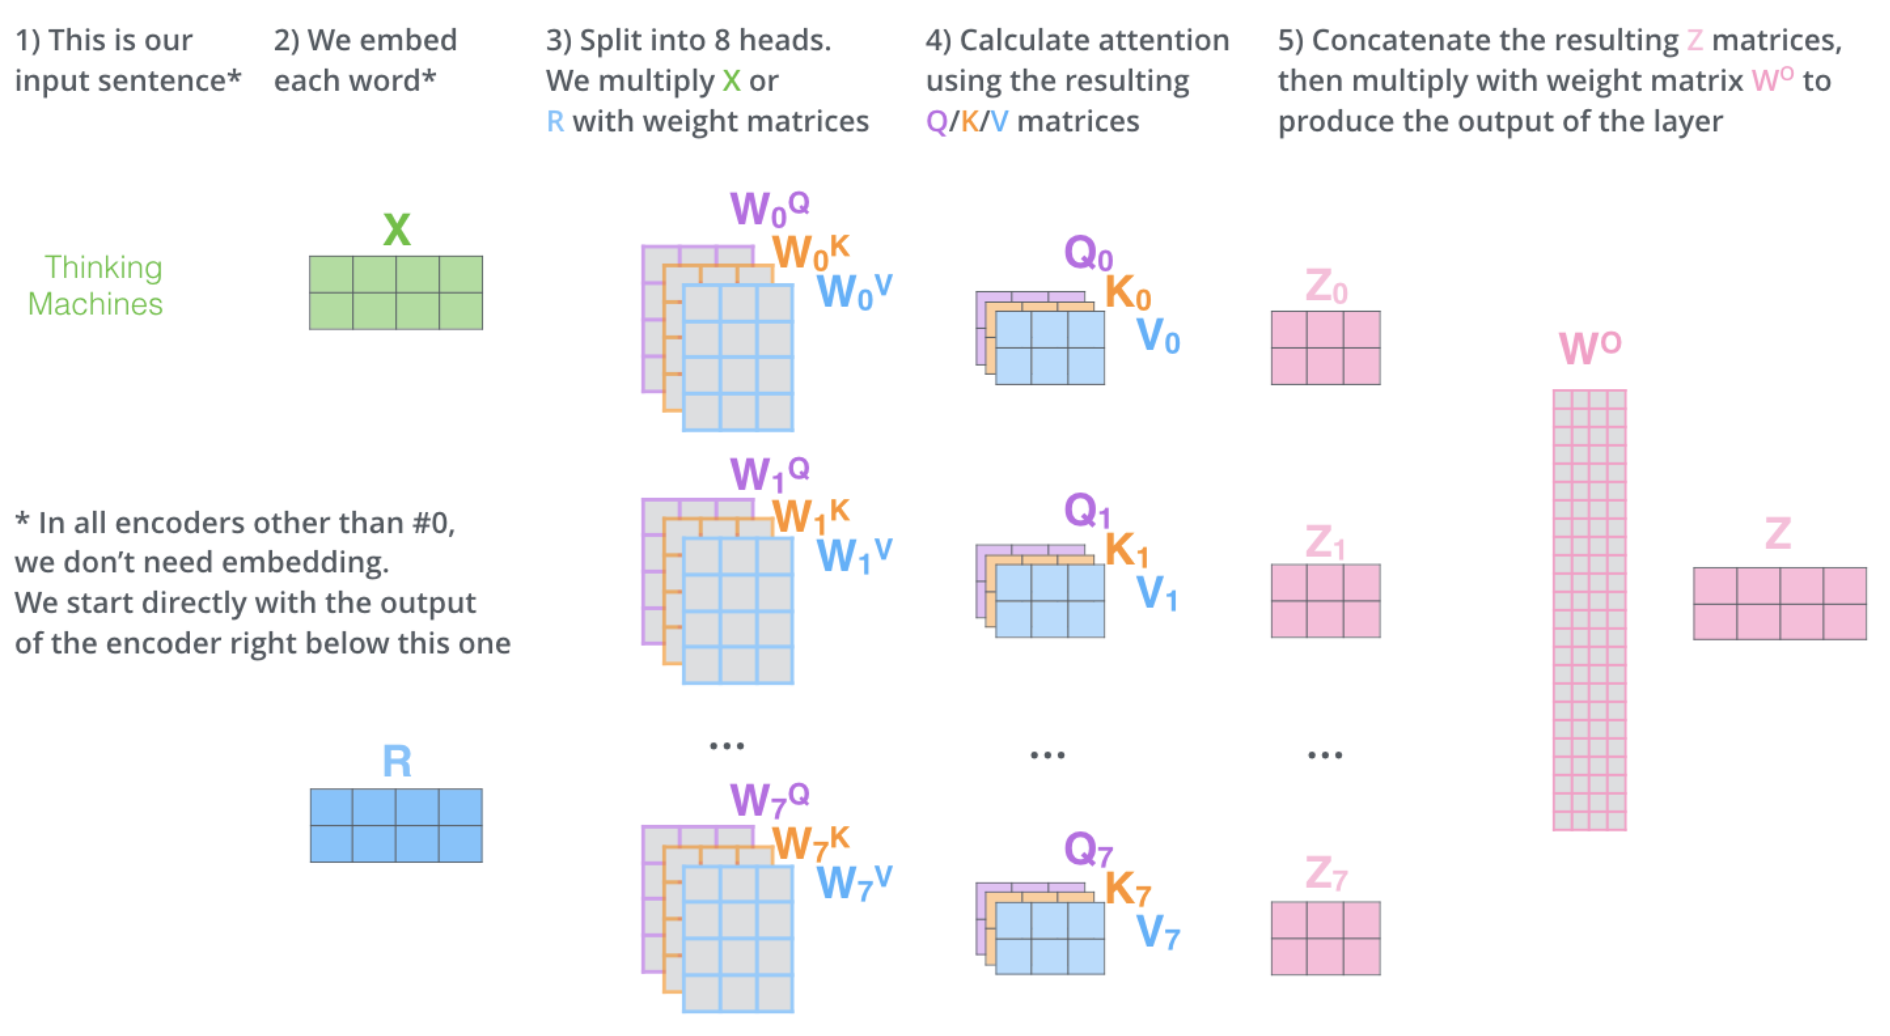
\includegraphics[width=\linewidth]{figures/multi_head_attention.png}
	\caption{Multi-head attention architecture \cite{Alammar2018}}
	\label{multi-head-attention}
\end{figure}

One can expand self-attention towards multi-head attention. In this configuration, each head produces its own query, key and value matrices and therefore its own self-attention output in its own representation subspace. The resulting hidden state is calculated by concatenating each hidden state output of the different heads and multiplying it with a contraction matrix that outputs a hidden state vector in its single-head dimensionality. Multi-head attention is needed to be able to better focus on multiple parts of the input sequence when encoding an input position, otherwise, it might happen that most of the focus is set on the input position itself. Vaswani et al. \cite{Vaswani2017} used 8 heads. \cite{Alammar2018, Vaswani2017}

Overall six layers of encoder and decoder components having individual weight matrices are stacked on top of each other to capture low-level as well as high-level features. The dimensionality of the hidden state is 512. Note that each position of the input sequence is encoded on an individual path through the transformer, which makes parallelization possible compared to \ac{LSTM} based architectures. \cite{Alammar2018, Vaswani2017}

The decoder uses almost the same architecture as the encoder but contains an additional multi-head attention component that integrates all the hidden state encodings from the encoder. Therefore the final hidden state encodings resulting from the top most encoder are transformed into key and value attention vectors and given to the integrating multi-head attention component of every decoder. Once again this helps to better focus on the relevant input positions for the current output position based on hidden state information extracted from the encoder. Note that the decoder works in a sequential manner again meaning that the input to the decoder are the already decoded sequence tokens of previous time steps, future input positions are masked away. The first multi-head attention component therefore captures inter-dependencies in the generated output sequence, the second one, the so-called encoder-decoder attention, enriches the hidden state encoding with the in\-for\-ma\-ti\-on given from the encoder hidden states. Finally, a linear layer mapping the hidden state vector to a logits vector with the dimensionality of the given output dictionary and a $softmax()$ function produce the output sequence using the greedy or beam search approach. The \textit{EOS} token symbolizes the end of the output to be generated. \cite{Alammar2018, Vaswani2017}

Input to the transformer are word embeddings also of fixed dimensionality of 512. Onto each word embedding a positional encoding following a specific pattern is added. These patterns are either learned or fixed and make sure that the distances of the input positions are projected onto the queue, key and value representations to be utilized during scaled dot-product attention. This also enables self-attention to be scaled to unseen lengths of sequences. Transformers usually contain an upper bound of sequence length to be pro\-ces\-sed, which is different from recurrent architectures that can process inputs of ar\-bi\-tra\-ry length. Input sequences are usually padded up until the specified sequence length, the used \textit{PAD} tokens are masked to be excluded from the self-attention components. \cite{Alammar2018, Vaswani2017}

% One is the total computational complexity per layer. Another is the amount of computation that can be parallelized, as measured by the minimum number of sequential operations required. The third is the path length between long-range dependencies in the network.

%\subsection{Other Techniques} \label{fundamentalsI}

%\begin{itemize}
%	\item NNs/SVMs: \url{https://bsb-eurasipjournals.springeropen.com/articles/10.1186/s13637-016-0042-0}
%	\item BiLSTM: \url{https://science.sciencemag.org/content/371/6526/284}
%\end{itemize}

\newpage
